\chapter{Fundamental Units and Laws of Electric Circuits}
\label{chap:fundamentals}
This chapter will introduce all of the foundational concepts of circuits. After you've read this chapter, almost everything else we cover will be derived from or otherwise based on these concepts. I'll start by introducing the concepts one-by-one using progressively more complicated examples, but then I'll recap the concepts more concisely at the end of the chapter.

\section{Schematics, Measurable Quantities, and Ohm's Law}
The majority of all circuits measurements are made using just four units---volts, amperes, ohms, and watts. To introduce these units, I will be referring to the simple circuit schematic of Figure \ref{resistorBatteryCircuit}.
\begin{figure}[h!]
\centering
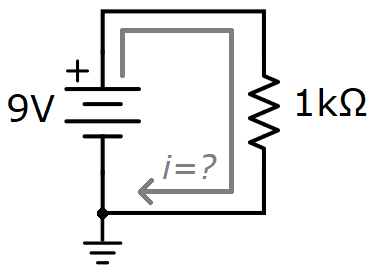
\includegraphics{figures/batteryResistorCircuit.png}
\caption{A simple circuit with a battery and a single resistor. The current in this circuit flows in the direction of the arrow.}
\label{resistorBatteryCircuit}
\end{figure}
Before we get into measurable quantities, let's look at the different elements of this schematic. In this circuit, there is a battery---represented by four horizontal lines and a plus sign---and a \textit{resistor}---the zig-zagged symbol on the right-hand side of the schematic. All of the straight lines that connect the elements in the circuit can be thought of as wire. All wires that are connected schematically have the same voltage value. Sections of wire are referred to as \textit{nodes}. A node is any part of a circuit that is described by a common voltage value. Nodes occupy the spaces between circuit elements.
\par
Volts represent energy per unit of charge, and in circuits they instigate the flow of electrons, which is current (measured in amperes). The battery is labelled ``9V'', meaning there is a 9 volt \textit{difference} between its positive and negative terminals. This also means there is a 9V difference between the nodes connected to its positive and negative terminals. The resistor is labelled ``1k$\Omega$'', meaning the resistance (or impedance) of that resistor is 1000 ohms. The gray arrow denotes the direction of current flow in this circuit; current typically flows out of the higher-voltage end of a source, through other elements in the circuit, and into the lower-voltage end of the source. 
\par
%Ohm's law
You are now probably wondering how the voltage of the battery, the resistance of the resistor, and the value of the current are all related. In order to determine the current flowing in this circuit, we will need to use \textbf{Ohm's Law}:
$$
V=i \cdot R
$$
In words, this law states that the voltage difference across (or the voltage ``dropped'' by) the resistor is equal to the value of the current flowing through the resistor (represented as $i$) multiplied by the resistance of the resistor. In the case of the circuit in Figure \ref{resistorBatteryCircuit}, the voltage across the resistor is defined by the battery as 9V. Since we know the value of the resistance is 1000$\Omega$, we can rearrange Ohm's law to find the value of the current flowing through the resistor:
$$
i = \frac{9\textrm{V}}{1000\Omega} = 0.009 \textrm{A}
$$
In words, this states that the current in question, $i$, is given by the voltage across the resistor, 9V, divided by the value of the resistor, 1000$\Omega$. This value is 0.009 \textit{Amperes}, which we will represent as ``A''. The value of the current flowing through the resistor is also the value of the current flowing out of the positive terminal of the battery and into the negative terminal of the battery, because current in a single branch of a circuit is always constant. Figure \ref{resistorBatteryCurrentCircuit} shows the fully-annotated schematic for this circuit.
\begin{figure}[h!]
\centering
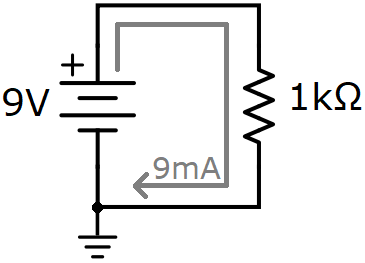
\includegraphics{figures/batteryResistorCurrentCircuit.png}
\caption{The circuit of Figure \ref{resistorBatteryCircuit}, with current labelled.}
\label{resistorBatteryCurrentCircuit}
\end{figure}
\par
%Watt's law
Having found the value of the current in this circuit, we have almost completely defined its behavior. However, remember that all circuits either power devices or condition signals, and even though this circuit is mostly instructive in purpose, let's assume that the whole point of this circuit is to provide power to the resistor. If that's the case, we need to determine how much power the resistor is receiving. To do so, we will rely on \textbf{Watt's Law}:
$$
P = i \cdot V
$$
In words, this states that the power (in Watts) dissipated or supplied by an element is given by the current flowing through that element multiplied by the voltage across that element. If the current is going in the direction of the voltage drop across the element---that is, into the terminal with greater voltage and out of the terminal with smaller voltage---then the element is dissipating that power. If the current flows in the opposite direction through the element, then that element is supplying power. We will see this soon.  By rearranging Ohm's Law and plugging it into Watt's law, we can generate two additional forms of Watt's Law:
$$
P = \frac{V^2}{R} = i^2\cdot R
$$
In analyzing circuits, you will sometimes find one of these forms of Watt's Law to be more useful than the others.
\par
Back to our circuit in Figure \ref{resistorBatteryCurrentCircuit}. If the voltage across the resistor is 9V and the current through the resistor is 9mA, then the power dissipated by the resistor is $9\textrm{mA}\cdot9\textrm{V} = 81\textrm{mW}$. Likewise, since there are 9V across the battery terminals and the current flowing through the battery is 9mA, the battery is \textit{supplying} 81mW.
\par
%KVL
Now we've completely defined all the possible quantities of this circuit and in so doing, we also introduced the concepts of \textit{voltage}, \textit{resistance}, \textit{current}, and \textit{power}, as well as \textit{Ohm's Law} and \textit{Watt's Law}. These are some of the most crucial concepts of the course, and there are really only a few more fundamental topics to introduce. Let's look at the slightly-more-complicated circuit of Figure \ref{simpleLED}.
\begin{figure}[h!]
\centering
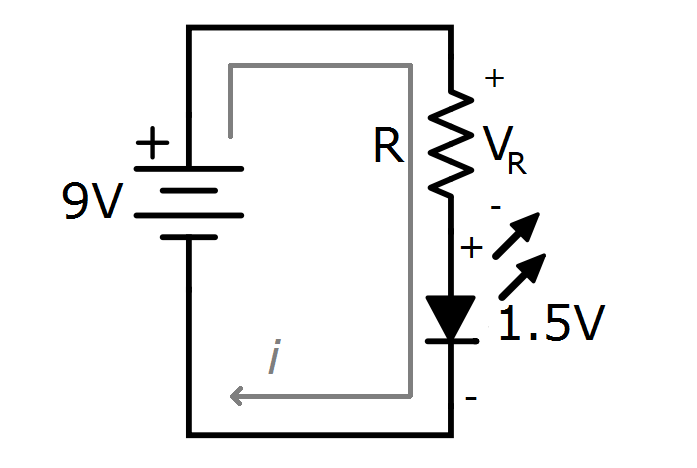
\includegraphics[width=10cm]{figures/LEDCircuit.png}
\caption{A circuit that lights up (read: provides power to) an LED.}
\label{simpleLED}
\end{figure}
This circuit is designed to light up (provide power to) a light emitting diode (LED) without destroying it. There are only three elements in this circuit: a battery, a resistor, and an LED (whose symbol looks like a big arrow pointing directly at a line, with little floating arrows above and to the right of it). The battery voltage is 9V, the resistor has a resistance of \textit{R}, and the LED, when operating, has a constant 1.5V across it. (I'm not going to describe how LEDs physically work in this class, but when an LED is emitting light, we can assume there is some constant voltage across it. 1.5V is a realistic voltage, but different LEDs can have different voltage values depending on the color and fabrication parameters of the LED.) The current, $i$, is shown in gray.  If I want to know how much power the LED is using, I just need to know the voltage across it and the current flowing through it. Then I can use Watt's Law to solve for the power being dissipated by the LED. For the circuit of Figure \ref{resistorBatteryCircuit}, I knew the voltage across the resistor and the resistance itself, and that information allowed me to use Ohm's law ($V=i \cdot R$) to find the current flowing through that circuit. In the circuit of Figure \ref{simpleLED} however, the voltage across the resistor is not given. To find it, we need to use \textbf{Kirchhoff's Voltage Law} (which I will refer to as \textbf{KVL} from now on):
$$
\textrm{For any loop in a circuit,} \sum\textrm{\{voltage added\}} = \sum\textrm{\{voltage dropped\}}
$$
In words, this states that if I trace through a complete loop of a circuit, I will encounter voltage drops and voltage increases, and for any such loop, the amount of voltage dropped will be equal to the amount of voltage added. If I trace clockwise through the circuit of Figure \ref{simpleLED} starting at the bottom left corner, I encounter the 9V increase of the battery, then an unspecified voltage drop across the resistor, and then the 1.5V drop across the LED, which takes me back to where I started. The increases in voltage and the voltage drops in that loop should sum to zero. Writing this out as an equation,
$$
9\textrm{V} - V_R - 1.5\textrm{V} = 0
$$
From this equation we see that the voltage drop across the resistor, $V_R = 7.5\textrm{V}$.
\par
With the voltage across the resistor determined, we can solve for the current flowing through the resistor and the LED in terms of the resistance, $R$. Remember that the purpose of this circuit is to provide power to the LED without destroying it. Let's assume that the LED can handle at most 30mW. If that's the case, then according to Watt's Law, the following expression must be true:
$$
1.5V \cdot i \leq 30\textrm{mW}
$$
To enforce this requirement, we must set $R$ so that the current does not exceed 30mW/1.5V, or 20mA. Using this expression for current and the fact that $V_R=7.5\textrm{V}$ along with Ohm's law, we can set a lower-bound on the range of allowable values for $R$ in the following way:
$$
7.5\textrm{V} = i \cdot R_{min} = 20\textrm{mA} \cdot R_{min},
$$
therefore
$$
R_{min} = \frac{7.5\textrm{V}}{20\textrm{mA}} = 375\Omega
$$
\par
So, in order for the LED in Figure \ref{simpleLED} to light up and not \textit{burn} up, the resistor value must be at least 375$\Omega$. If you followed along with this example, congratulations! You just experienced a taste of electric circuit design!
\par
%KCL
There is one last fundamental law to introduce, and to do so we will look at the circuit of Figure \ref{twoLEDs}.
\begin{figure}[h!]
\centering
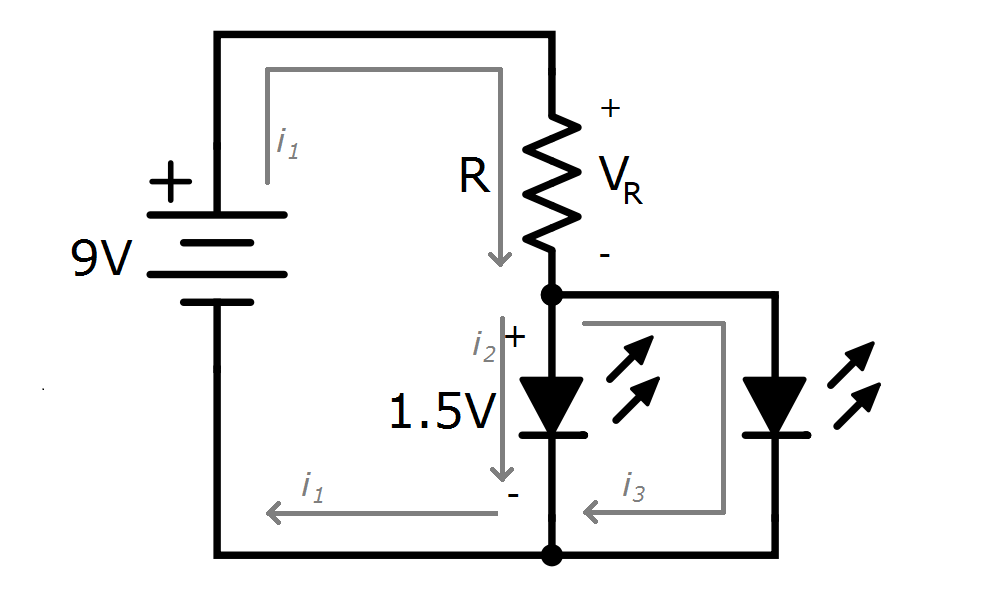
\includegraphics[width=12cm]{figures/twoLEDsCircuit.png}
\caption{A circuit that lights up two LEDs.}
\label{twoLEDs}
\end{figure}

This circuit is comprised of a battery, a resistor, and two LEDs. As before, the voltage across both of the LEDs is 1.5V, and KVL tells us that the voltage across the resistor must be 7.5V. However, this circuit has more than just one full loop. The dot between the resistor and the two LEDs indicates that all three wires converging there are connected and thus form a \textit{node}. At that node, current $i_1$ enters from the resistor branch and currents $i_2$ and $i_3$ exit through the two LED branches. We can relate these three currents usign \textbf{Kirchhoff's Current Law} (which I will refer to as \textbf{KCL} from now on): 
$$
\textrm{At any node in a circuit,} \sum\textrm{\{current entering\}} = \sum\textrm{\{current leaving\}}
$$
In words, this means that the amount of current flowing into a node must be equal the amount of current flowing out of that node. In our circuit, this means that $i_1=i_2+i_3$. Let's assume that both LEDs are identical, and therefore the current flowing through each LED is the same. In that case, $i_2=i_3$. Let's also assume that we need to enforce the same constraints on the power delivered to each LED as before---$P_{LED}\leq30\textrm{mW}$. Therefore, the current flowing through each LED must be constrained to be 20mA or less (we'll define $i_{2,max}=20\textrm{mA}$ and $i_{3,max}=20\textrm{mA}$). If we assume that each of these currents is at its maximum value, then $i_2=i_3=20\textrm{mA}$ and according to KCL, the maximum value for the current flowing through the resistor in this circuit $i_{1,max}=i_{2,max}+i_{3,max}=40\textrm{mA}$. As was the case in our analysis of the circuit in Figure \ref{simpleLED}, this maximum current value places a constraint on the possible resistance values of our resistor; given the fact that the voltage across the resistor is set at 7.5V, according to Ohm's Law, $R_min=7.5V/i_{1,max}=187.5\Omega$. This is half of the minimum resistance value we found for the circuit of Figure \ref{simpleLED}; why do you think that is?
\section{Recap: The Fundamentals}
In the previous section, I introduced several fundamental concepts without dwelling too much on definitions. I want to ennumerate and concisely define each of these concepts here again:
\begin{description}
\item[Voltage] is measured in \textit{Volts} and is defined as energy per unit charge. Dimensionally, 1V=1J/1C. A \textit{node} in a circuit is a section that has a common voltage. We often will refer to voltage \textit{across} an element; by this, we mean the \textit{difference} between the voltages at the two ends of that element. 
\item[Current] is measured in \textit{Amperes} (or just \textit{Amps}, and is defined as the flow of charge through an element or elements. Dimensionally, 1A=1C/1s. Current that flows through a single branch has a constant value at all points along that branch.
\item[Resistance] is measured in \textit{Ohms}, and it relates the voltage across a resistor to the current flowing through that resistor. Dimensionally, $1\Omega$=1V/1A. Resistance is the real (as opposed to imaginary)  part of a broader relationship between current and voltage known as \textit{impedance}, which we will introduce later in the course.
\item[Power] is measured in \textit{Watts}, and is defined as energy supplied or dissipated over time. Dimensionally, 1W=1V$\cdot$1A.\footnote{1W=1J/1s of course, but the definition above is generally more useful for this course. The standard definition can be derived from 1W=1V$\cdot$1A without too much effort.} Power in circuits is typically supplied by voltage or current sources and dissipated by resistors.
\item[Ohm's Law] is related to resistance, and it states that the value of the voltage across a resistive element is equal to the value of the current flowing through that element multiplied by the resistance of that element:
$$V=i \cdot R$$
\item[Watt's Law] is the name for the law that relates power supplied or dissipated by a circuit element to the current flowing through that element and the voltage across that element. Through the use of Ohm's Law, several forms of Watt's Law can be derived: 
$$
P = i \cdot V = i^2 \cdot R = \frac{V^2}{R}
$$
\item[Kirchhoff's Voltage Law (KVL)] states that around any loop in a circuit, the voltage added is equal to the voltage dropped:
$$\textrm{Around a loop in a circuit,  }\sum{V_{added}} = \sum{V_{dropped}}$$
This law is an expression of the concept of conservation of energy; all the energy delivered to a circuit must be dissipated by that circuit.
\item[Kirchhoff's Current Law(KCL)] states that at any node in a circuit, the current flowing in is equal to the current flowing out:
$$\textrm{At any node in a circuit,  }\sum{i_{in}} = \sum{i_{out}}$$
This law is an expression of the concept of conservation of mass; however many electrons flow into a node must also flow out of that node.
\end{description}
\par
These concepts may seem overwhelming all at once, but everything we do now will rely on these. If you read this whole chapter, you have now seen \textit{every} fundamental concept pertaining to electric circuits.
